\documentclass{article}
\usepackage[utf8]{inputenc}
\usepackage{listings}
\usepackage{graphicx}
\usepackage{float}
\usepackage{xcolor}
\usepackage{geometry}
\usepackage{CJKutf8}
\usepackage{diagbox}

\geometry{a4paper,scale=0.8}
\lstset{
    basicstyle          =   \sffamily,        
    keywordstyle        =   \bfseries,         
    commentstyle        =   \rmfamily\itshape, 
    stringstyle         =   \ttfamily, 
    flexiblecolumns,               
    numbers             =   left,  
    showspaces          =   false, 
    showstringspaces    =   false,
    captionpos          =   t,     
    frame               =   lrtb, 
}

\lstdefinestyle{Python}{
    language        =   Python, 
    basicstyle      =   \zihao{-5}\ttfamily,
    numberstyle     =   \zihao{-5}\ttfamily,
    keywordstyle    =   \color{blue},
    keywordstyle    =   [2] \color{teal},
    stringstyle     =   \color{magenta},
    commentstyle    =   \color{red}\ttfamily,
    breaklines      =   true,  
    columns         =   fixed,  
    basewidth       =   0.5em,
}

\title{\bf\Large  概率论与数理统计 第2次作业}
%%%%%%%%%%%%%%%%%%%%%%%%%%%%%%%%%%%%%%
%% DON'T forget to change this part %%
\author{\bf Name: 宋昊原 \qquad Student ID: 2022010755}
%%%%%%%%%%%%%%%%%%%%%%%%%%%%%%%%%%%%%%

\begin{document}
\begin{CJK}{UTF8}{gbsn}
\maketitle
\section{三元容斥}
$$ A+B+C=(A+B)^{c}C+(A+B)C^{c}+(A+B)C $$
$$ =A^{c}B^{c}C+(A^{c}B+AB^{c}+AB)C^{c}+(A^{c}B+AB^{c}+AB)C $$
$$ =A^{c}B^{c}C+A^{c}BC^{c}+AB^{c}C^{c}+ABC^{c}+A^{c}BC+AB^{c}C+ABC $$
将上述七项分别记作$F_{1}$至$F_{7}$,则类似地有
$$ A=F_{3}+F_{4}+F_{6}+F_{7} $$
$$ B=F_{2}+F_{4}+F_{5}+F_{7} $$
$$ A=F_{1}+F_{5}+F_{6}+F_{7} $$
$$ AB=F_{4}+F_{7} $$
$$ BC=F_{5}+F_{7} $$
$$ AC=F_{6}+F_{7} $$
$$ ABC=F_{7} $$
$F_{1}$至$F_{7}$两两互斥,故有
$$ P(A+B+C)=\sum\limits_{i=1}^{7} P(F_{i})=P(A)+P(B)+P(C)-P(AB)-P(BC)-P(AC)+P(ABC) $$
\section{条件概率}
分别证明三条概率需要满足的三条原理.
\subsection{$P(A|B)>=0$}
$\forall A\in \mathcal{F}$,有$P(AB)\geq 0$,又由题设,$P(B)>0$,故有
$$ P(A|B)=\frac{P(AB)}{P(B)}\geq 0$$
\subsection{$P(\Omega|B)=1$}
$$ P(\Omega|B)=\frac{P(\Omega B)}{P(B)}=\frac{P(B)}{P(B)}=1 $$
\subsection{加法原理}
$\forall A_{i},A_{j},A_{i}A_{j}=\emptyset $,有$(A_{i}B)(A_{j}B)=A_{i}A_{j}B=\emptyset B=\emptyset $,于是任何$A_{i}B,A_{j}B$互斥. 进而有
$$ \sum\limits_{i=1}^{\infty} P(A_{i}|B)=\sum\limits_{i=1}^{\infty} \frac{P(A_{i}B)}{P(B)} $$
$$ =\frac{\sum\limits_{i=1}^{\infty} P(A_{i}B)}{P(B)} $$
$$ =\frac{P(\sum\limits_{i=1}^{\infty} A_{i}B)}{P(B)} $$
$$ =\frac{P((\sum\limits_{i=1}^{\infty} A_{i})B)}{P(B)} $$
$$ =P(\sum\limits_{i=1}^{\infty} A_{i}|B) $$
\section{互斥事件和独立事件}
\subsection{}
不正确. 当$P(A)<1$且$A=B$时,$P(A|B)=P(A|A)=1>P(A)$.
\subsection{}
不正确. 当$B=\emptyset$时,显然$A$与$B$互斥,而$P(AB)=P(A)P(B)=0$.
\subsection{}
不正确. 当$A=\emptyset$且$P(B)P(C)\neq P(BC)$时,也有$P(ABC)=P(A)P(B)P(C)=0$.
\section{反直觉的独立性}
掷两个骰子可能的点数和及对应的样本点数如下表:\\\\
\begin{tabular}{l|c|c|c|c|c|c|c|c|c|c|c}
	点数和&2&3&4&5&6&7&8&9&10&11&12\\
	\hline
	样本点数&1&2&3&4&5&6&5&4&3&2&1
\end{tabular}\\\\
据表有
$$ P(A_{2})=\frac{1+3+5+5+3+1}{36}=\frac{1}{2} $$
$$ P(A_{3})=\frac{2+5+4+1}{36}=\frac{1}{3} $$
$$ P(A_{5})=\frac{4+3}{36}=\frac{7}{36} $$
$$ P(A_{2}A_{3})=P(A_{6})=\frac{5+1}{36}=\frac{1}{6} $$
$$ P(A_{10})=\frac{3}{36}=\frac{1}{12} $$
故
$$ P(A_{2}A_{3})=P(A_{2})P(A_{3}) $$
而
$$ P(A_{2}A_{5})\neq P(A_{2})P(A_{5}) $$
于是$A_{2}$和$A_{3}$独立,$A_{2}$和$A_{5}$不独立.
\section{独立和条件独立}
\subsection{独立并不意味着条件独立}
掷一个骰子,设$A_{1}$表示点数为偶数,$A_{2}$表示点数为3的倍数,$B$表示点数大于等于4. 我们有:
$$ P(A_{1})=\frac{1}{2} $$
$$ P(A_{2})=\frac{1}{3} $$
$$ P(A_{1}A_{2})=\frac{1}{6} $$
$$ P(A_{1}|B)=\frac{2}{3} $$
$$ P(A_{2}|B)=\frac{1}{3} $$
$$ P(A_{1}A_{2}|B)=\frac{1}{3} $$
可见$A_{1}$与$A_{2}$独立,但并不关于$B$条件独立.
\subsection{条件独立并不意味着独立}
设$0<P(B)<1$,则$B$与$B$总是不独立的,但$B$与$B$关于$B$独立.
\section{小概率事件}
设$A_{i}$表示第$i$次试验中事件$A$不发生. 则
$$P(A_{i})=1-\epsilon $$
前$n$次试验中发生一次的概率为
$$ 1-\prod\limits_{i=1}^{n} P(A_{i})=1-(1-\epsilon)^{n} $$
故试验迟早发生一次的概率为
$$ \lim_{n\to \infty}1-(1-\epsilon)^{n}=1-0=1 $$
\section{红黑卡片}
设$A$为向上的面为红色,$B_{1}$为选中全黑卡片,$B_{2}$为选中全红卡片,$B_{3}$为选中双色卡片.
\\则$B_{1}$,$B_{2}$,$B_{3}$构成对样本空间$\Omega$的一个等概率划分.
\\我们有
$$ P(A|B_{1})=0 $$
$$ P(A|B_{2})=1 $$
$$ P(A|B_{3})=\frac{1}{2} $$
根据Bayes公式,我们有
$$ P(B_{3}|A)=\frac{P(A|B_{3})P(B_{3})}{P(A|B_{1})P(B_{1})+P(A|B_{2})P(B_{2})+P(A|B_{3})P(B_{3})} $$
$$ =\frac{\frac{1}{2}\times \frac{1}{3}}{0\times \frac{1}{3}+1\times \frac{1}{3}+\frac{1}{2}\times \frac{1}{3}} $$
$$ =\frac{1}{3} $$
即此时另一面是黑色(即$B_{3}$发生)的概率是$\frac{1}{3}$
\section{抓阄}
两种方案都公平.
\subsection{抓完同时打开的方案}
这种方案下,每个人抓到“中”的概率都是先验概率$\frac{1}{n}$,公平.
\subsection{边抓边打开的方案}
这种方案下,每个人抓到“中”的概率会随着之前阄的打开变成后验概率,下面我们根据这个逻辑讨论每个人中签的全概率. 设第$i$个人中签为事件$A_{i}$. 
\\首先,第一个人中签与先验后验无关,$P(A_{1})=\frac{1}{n}$
\\第二个人中签的条件是第一个人没中签,而此时的条件概率为$\frac{1}{n-1}$,则有
$$ P(A_{2})=P(A_{1}^{c})P(A_{2}|A_{1}^{c})=\frac{8}{9}\times \frac{1}{8}=\frac{1}{9} $$
类似地
$$ P(A_{i})=P(A_{1}^{c})P(A_{2}^{c}|A_{1}^{c})...P(A_{i-1}^{c}|A_{1}^{c}...A_{i-1}^{c})P(A_{i}|A_{1}^{c}A_{2}^{c}...A_{i-1}^{c}) $$
$$ =\frac{n-1}{n}\times \frac{n-2}{n-1}\times ...\times \frac{n-i+1}{n-i+2}\times \frac{1}{n-i+1}$$
$$ =\frac{1}{n} $$
因此每个人中签的概率均为$\frac{1}{n}$,方案公平.
\section{手术诊断}
设事件$A$表示小明患病,$B$表示检验阳性,则先验概率$P(A)=0.6$,条件概率$P(B|A)=1$,$P(B|A^{c})=0.3$. 根据Bayes公式,我们有
$$ P(A|B)=\frac{P(B|A)P(A)}{P(B|A)P(A)+P(B|A^{c})P(A^{c})} $$
$$ =\frac{1\times 0.6}{1\times 0.6+0.3\times 0.4} $$
$$ =\frac{5}{6}>0.8 $$
故医生应该建议手术.
\section{不要赌博}
本题我的做法参考了William Feller著《概率论及其应用》中对随机徘徊和破产问题的讨论,加以整理得到.
\subsection{破产的概率}
设此人在初始资金为$r$时会输光离场的概率为$q(r)$(为了严谨起见做此声明:这里的“会破产的概率”是$m$轮内会破产的概率对$m\to \infty$的极限,$m$轮内会破产的概率是单调不减的,故此极限存在).
\\可以写出$q_{r}$满足的方程:
\\
\begin{equation}
    q_{r}=\left\{
    \begin{array}{cl}
    1  &  r=0\\
    pq_{r+1}+(1-p)q_{r-1} & 0<r<n\\
    0  &  r=n\\
    \end{array}\right.
    \end{equation}
\\考虑当$0<r<n$时的差分方程:\\
\begin{equation}
    q_{r}=pq_{r+1}+(1-p)q_{r-1}
\end{equation}
\\假如我们已经找到了方程(2)的两个线性无关的特解$q_{1,r}$和$q_{2,r}$,由于$q_{r}$可以由$q_{0}$和$q_{1}$确定,方程(2)的解空间维数为2,故$q_{r}=Aq_{1,r}+Bq_{2,r}$是全部可能的解,进而可以待定系数法根据边界条件求出对应的概率解.
\\\\考虑$p\neq \frac{1}{2}$的情形,我们可以找到(2)的两个线性无关的特解$q_{r}=1$和$q_{r}=(\frac{1-p}{p})^{r}$,故可能的解表达为:
$$ q_{r}=A+B(\frac{1-p}{p})^{r} $$
代入边界条件$q_{0}=1$和$q_{n}=0$解得:
$$ q_{r}=\frac{(\frac{1-p}{p})^{n}-(\frac{1-p}{p})^r}{(\frac{1-p}{p})^{n}-1} $$
\\\\考虑$p=\frac{1}{2}$的情形,两个线性无关特解为$q_{r}=1$和$q_{r}=r$,于是类似手段可以得到满足边界条件的解:
$$ q_{r}=1-\frac{r}{n} $$
\\\\综上所述,破产的概率为:
\\
\begin{equation}
    q_{k}=\left\{
    \begin{array}{cl}
        \frac{(\frac{1-p}{p})^{n}-(\frac{1-p}{p})^k}{(\frac{1-p}{p})^{n}-1} & p\neq \frac{1}{2} \\
        1-\frac{k}{n} & p=\frac{1}{2}\\
    \end{array}\right.
\end{equation}
\subsection{极限情况讨论}
$p\leq 0.5$时,对$n\to \infty$取极限,有$q_{k}=1$,与$k$无关.
\section{生物灭亡}
设一个此种生物最终灭亡的概率是$p$.
\\在此说明:这里$p$指的是$m$分钟后这一个生物及其全部可能后代全部死亡的概率对$m\to \infty$的极限. 由于这个概率应当对$m$单调不减而有上界$1$,故此极限存在.
\\考虑接下来等可能发生的三个事件:生物死亡,存活1个,或分裂成2个,其概率均为$\frac{1}{3}$,而这三种情形下的该生物及其可能后代全部死亡的概率分别为$1$,$p$,$p^{2}$(这里已经利用了每个此生物个体在每一时刻的命运相互独立的条件).
\\故我们有
$$ p=\frac{1}{3}+\frac{1}{3}p+\frac{1}{3}p^{2} $$
解得唯一解$p=1$,故此生物经过足够长的时间后必然灭亡.
\\\\
\textbf{注记}
\\若三个概率分别改为$\frac{1}{3},0,\frac{2}{3}$,则可以解出$p=\frac{1}{2}$和$p=1$两个解,此时应取小者. 具体原因有待进一步讨论.
\section{治疗方案}
设两种治疗方案治愈该患者分别为事件$W_{1}$和$W_{2}$,患者患A、B、C病设为事件$A$、$B$、$C$.
(注:这里$W_{1}$和$W_{2}$应当认为属于不同的概率空间,它们不会同时被选择)
\\$A$、$B$、$C$构成对样本空间的一个分割,则有
\\
$$ P(W_{1})=P(W_{1}|A)P(A)+P(W_{1}|B)P(B)+P(W_{1}|C)P(C) $$
$$ =0.8\times 0.8+0.05\times 0.1+0.1\times 0.1=0.655 $$
$$ P(W_{2})=P(W_{2}|A)P(A)+P(W_{2}|B)P(B)+P(W_{2}|C)P(C) $$
$$ =0.6\times 0.8+0.9\times 0.1+0.9\times 0.1=0.66 $$
\\
故$P(W_{1})<(W_{2})$,纯从治愈率高的角度应当采取乙方案.
\\而考虑到该患者大概率患的是A病,而甲方案对A病治愈率很高,也可以推荐甲方案. 
\\用$p_{ij}$表示该患者依次经过$i$,$j$两次治疗后治愈的概率,考虑两次治疗后治愈的概率:
$$ p_{11}=0.655+0.16\times 0.8+0.095\times 0.05+0.09\times 0.1=0.797 $$
$$ p_{12}=0.655+0.16\times 0.6+0.095\times 0.9+0.09\times 0.9=0.918 $$
$$ p_{21}=0.66+0.32\times 0.8+0.01\times 0.05+0.01\times 0.1=0.918 $$
$$ p_{22}=0.66+0.32\times 0.6+0.01\times 0.9+0.01\times 0.9=0.870 $$
这可以看出,实际上无论先使用甲方案还是乙方案,为了让两次完成治愈的概率较大,如果第一次没有治愈,第二次都应该选择另一种方案.
\section{摸球}
\subsection{}
$$ P(B_{1})=\frac{1}{2}P(B_{1}|U_{1})+\frac{1}{2}P(B_{1}|U_{2})=\frac{6}{10}=\frac{3}{5} $$
$$ P(U_{1}|B_{1})=\frac{\frac{1}{2}P(B_{1}|U_{1})}{P(B_{1})}=\frac{2}{3} $$
$$ P(U_{1})=\frac{1}{2} $$
$P(U_{1}|B_{1})>P(U_{1})$,这是因为$U_{1}$中黑球所占比例大于$U_{2}$,因此如果摸出了黑球,更有理由认为是从$U_{1}$中摸出的.
\subsection{}
若将第一个球放回,第二个球与第一个球无区别,故
$$ P(B_{2})=P(B_{1})=\frac{3}{5} $$
若不放回,则需要考虑选择$U_{1}$还是$U_{2}$.
$$ P(B_{2}|U_{1})=P(B_{2}|U_{1}B_{1})P(B_{1}|U_{1})+P(B_{2}|U_{1}B_{1}^{c})P(B_{1}^{c}|U_{1}) $$
$$ =\frac{3}{4}\times \frac{4}{5}+\frac{4}{4}\times \frac{1}{5}=\frac{4}{5} $$
$$ P(B_{2}|U_{2})=P(B_{2}|U_{2}B_{1})P(B_{1}|U_{2})+P(B_{2}|U_{2}B_{1}^{c})P(B_{1}^{c}|U_{2}) $$
$$ =\frac{1}{4}\times \frac{2}{5}+\frac{2}{4}\times \frac{3}{5}=\frac{2}{5} $$
于是
$$ P(B_{2})=P(B_{2}|U_{1})P(U_{1})+P(B_{2}|U_{2})P(U_{2})=\frac{4}{5}\times \frac{1}{2}+\frac{2}{5}\times \frac{1}{2}=\frac{3}{5}$$
故仍有$P(B_{2})=P(B_{1})$.
\\事实上,无论最开始选取的袋子是哪个袋子,由于不知道第一次摸球的结果,无论放回还是不放回,第一次摸球和第二次摸球摸到黑球的概率都是一样的. 因此无论放回还是不放回,都有$P(B_{2})=P(B_{2})$.
\subsection{}
此时$B_{1}$已经发生,根据第一问,有
$$P(U_{1}|B_{1})=\frac{2}{3}$$
$$P(U_{2}|B_{1})=1-P(U_{1}|B_{1})=\frac{1}{3}$$
$$P(B_{2}|B_{1})=P(B_{2}|U_{1}B_{1})P(U_{1}|B_{1})+P(B_{2}|U_{2}B_{1})P(U_{2}|B_{1})$$
$$ =\frac{4}{5}\times \frac{2}{3}+\frac{2}{5}\times \frac{1}{3}=\frac{2}{3} $$
于是,$P(B_{2}|B_{1})>P(B_{2})$,此时因为已知第一个球摸出黑球,第一问中已做解释,此时实际提高了取到$U_{1}$袋的后验概率,进一步也就提高了第二次摸到黑球的概率.
\subsection{}
$$P(U_{1}|B_{1}B_{2}...B_{n})=\frac{P(B_{1}B_{2}...B_{n}|U_{1})P(U_{1})}{P(B_{1}B_{2}...B_{n}|U_{1})P(U_{1})+P(B_{1}B_{2}...B_{n}|U_{2})P(U_{2})} $$
$$=\frac{(\frac{4}{5})^{n}\times \frac{1}{2}}{(\frac{4}{5})^{n}\times \frac{1}{2}+(\frac{2}{5})^{n}\times \frac{1}{2}}=\frac{(\frac{4}{5})^{n}}{(\frac{4}{5})^{n}+(\frac{2}{5})^{n}} $$
于是
$$P(U_{2}|B_{1}B_{2}...B_{n})=1-P(U_{1}|B_{1}B_{2}...B_{n})=\frac{(\frac{2}{5})^{n}}{(\frac{4}{5})^{n}+(\frac{2}{5})^{n}}$$
故
$$P(B_{n+1}|B_{1}...B_{n})=P(B_{n+1}|B_{1}...B_{n}U_{1})P(U_{1}|B_{1}...B_{n})+P(B_{n+1}|B_{1}...B_{n}U_{2})P(U_{2}|B_{1}...B_{n})$$
$$=\frac{4}{5}\times\frac{(\frac{4}{5})^{n}}{(\frac{4}{5})^{n}+(\frac{2}{5})^{n}}+\frac{2}{5}\times\frac{(\frac{2}{5})^{n}}{(\frac{4}{5})^{n}+(\frac{2}{5})^{n}}=\frac{(\frac{4}{5})^{n+1}+(\frac{2}{5})^{n+1}}{(\frac{4}{5})^{n}+(\frac{2}{5})^{n}}$$
令$n\to \infty$,有
$$\lim_{n\to \infty}P(B_{n+1}|B_{1}...B_{n})=\frac{4}{5}$$
事实上,随着连续摸到黑球的次数增多,对选到的袋子是$U_{1}$的后验概率就越来越大,如果连续无数次摸到黑球,则此后验概率就是$1$,于是摸到黑球的概率就是$P(B_{1}|U_{1})=\frac{4}{5}$.
\subsection{}
上一问已经进行了计算:
$$P(U_{1}|B_{1}...B_{n})=\frac{(\frac{4}{5})^{n}}{(\frac{4}{5})^{n}+(\frac{2}{5})^{n}}$$
同时
$$\lim_{n\to \infty}P(U_{1}|B_{1}...B_{n})=1$$
这个理解在上一问也有提到,因为1号袋中黑球比例高于2号袋,因此如果连续摸到黑球的数目足够多,则选到1号袋的后验概率会逐渐增加直到增加到1.
\section{对赌}
\subsection{}
假设100元中用$x$元跟甲对赌,用$100-x$元跟乙对赌,则若A获胜,会获利$-x+(100-x)\times\frac{15}{10}=150-\frac{5}{2}x$元,若B获胜,会获利$x\times\frac{20}{5}-(100-x)=5x-100$元.
要想必定获利,要求上述两个获利值都为正,即
$$150-\frac{5}{2}x>0$$
且
$$5x-100>0$$
解得
$$20<x<60$$
故要想必定获利,不能只和一家对赌,而要出20至60元与甲赌,出40至80元与乙赌.
\subsection{}
甲、乙的主观概率应满足两人的期望收益为0. 故
$$-20P_{1}(B)+5(1-P_{1}(B))=0$$
$$-15P_{2}(A)+10(1-P_{2}(A))=0$$
解得
$$P_{1}(B)=\frac{1}{5}$$
$$P_{2}(A)=\frac{2}{5}$$
于是
$$P_{1}(B)+P_{2}(A)=\frac{3}{5}<1$$
这说明,两人都对自己支持的队伍的胜率有过高的估计,这导致他们愿意出大金额对赌,从而使得存在与他们同时对赌而必定获利的方式. 若$P_{1}(B)+P_{2}(A)\geq 1$,则不会有这种情况出现.
\section{计算机实验:掷硬币}
\begin{figure}[htbp]
    \centering
    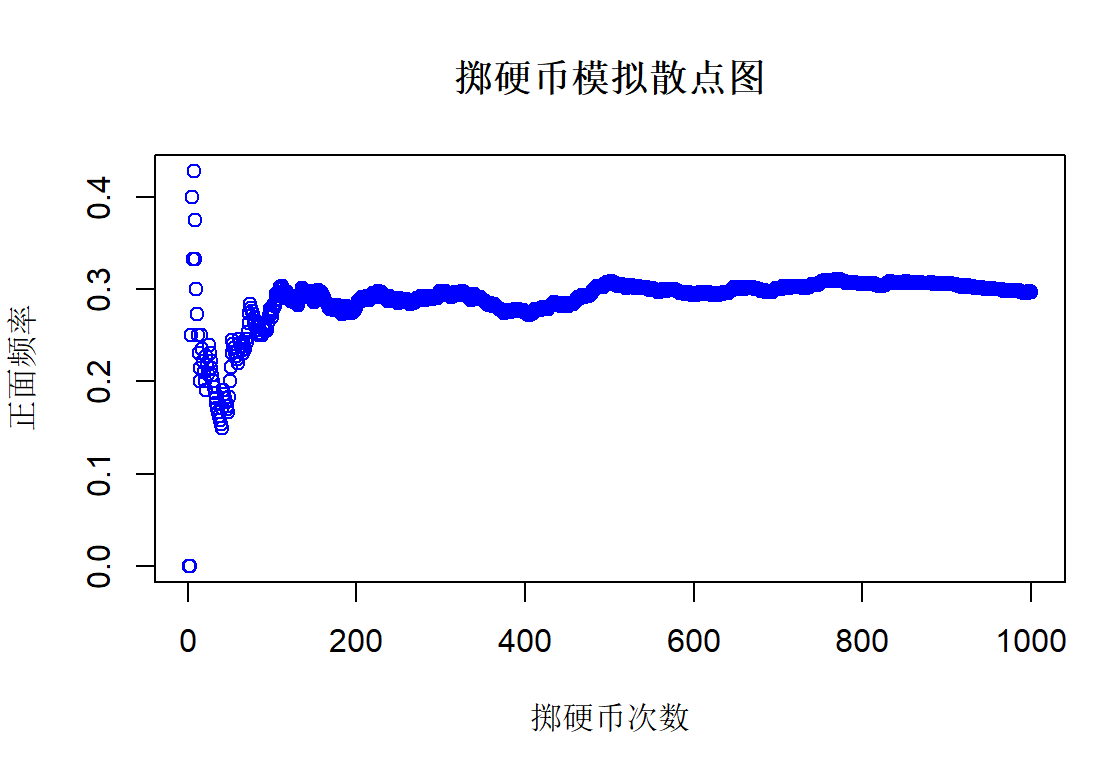
\includegraphics[scale=0.7]{plot1.png}
    \caption{一次试验的相对频数散点图}
    \label{1}
\end{figure}
\begin{figure}[htbp]
    \centering
    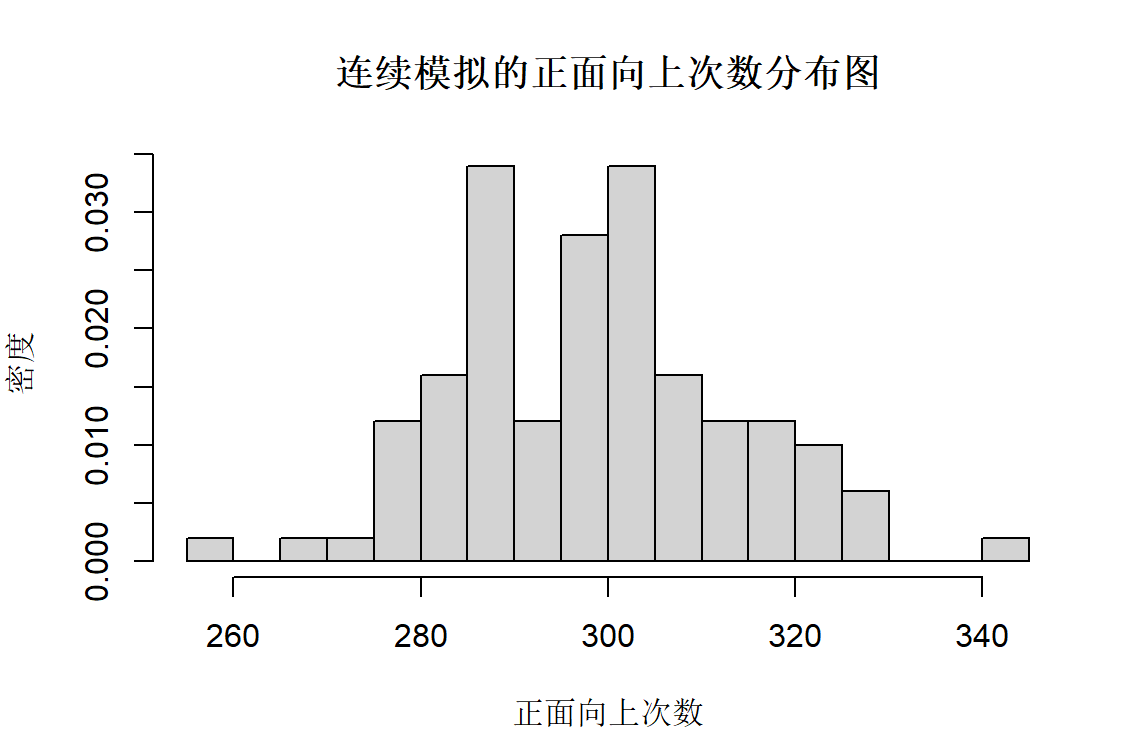
\includegraphics[scale=0.7]{plot2.png}
    \caption{多次试验的正面向上次数直方图}
    \label{2}
\end{figure}
\begin{figure}[htbp]
    \centering
    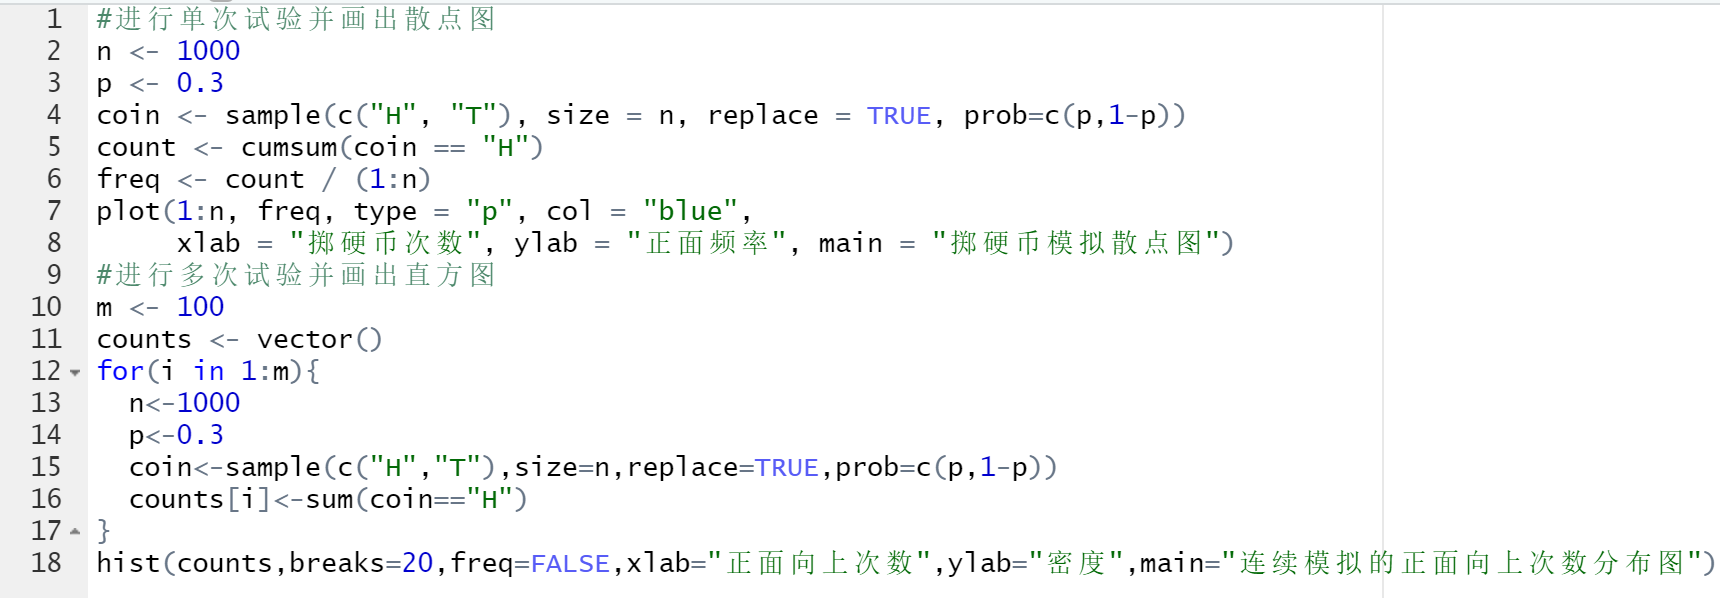
\includegraphics[scale=0.5]{code.png}
    \caption{完成实验的R语言代码}
    \label{3}
\end{figure}
\end{CJK}
\end{document}